\documentclass[]{article}
\usepackage{pgfplots}

%opening
\title{Real Numbers}
\date{February 2, 2016}
\author{}

\begin{document}

\maketitle

\tableofcontents
\pagebreak

\section{Types of Numbers}
\subsection{Whole Numbers}
$$ (0,1,2,3,4)$$
\subsection{Natural Numbers}
These are also known as "counting numbers". $$(1,2,3,4...)$$
\subsection{Integers}
Any whole number that does not have decimal or fractional part.
$$(-3,-2,-1,0,1,2,3,4...)$$
\subsection{Even Numbers}
These numbers can be easily divisible by two.
$$(2,4,6,8...)$$
\subsection{Odd numbers}
Number NOT easily divisible by two.
$$(1,3,5,7...)$$
\subsection{Prime Number}
Numbers that are not evenly divisible by themselves or one.\footnote{Two is the only even prime number.}
$$(2,3,5,7,11,13,17,19,23...)$$
\subsection{Irrational Number}
A decimal number that goes on forever and does not repeat. \footnote{$\pi$ is probably the most famous irrational number.}
$$(3.1415926..., \sqrt 2)$$
\subsection{Rational Number}
The opposite of an irrational number. These number will eventually end or start repeating.
$$(3.5,3.33333...)$$
\subsection{Number Line}
All real numbers can be found on the number line.

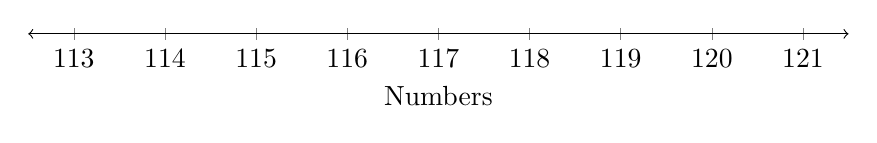
\begin{tikzpicture}
\begin{axis}[
axis y line=none,
axis lines=left,
axis line style={<->},
xmin=112.5,
xmax=121.5,
width=12cm,
height=4cm,
ymin=0,
ymax=1,
xlabel= Numbers,
scatter/classes={o={mark=*}},
restrict y to domain=0:1,
xtick={113,114,...,121}
]
\end{axis}
\end{tikzpicture}

\subsection{Examples of real Numbers}
$$\sqrt {81} = 9 $$
$$\sqrt {49} = 7 $$
$$\sqrt {25} = 5 $$
$$\sqrt {NegativeNumber} = NOT REAL$$ \footnote{Imaginary Numbers are for another lesson.}

\section{Word Problems}
\subsection{Adding}
These are words that you will want to recognize as additoin when reading a Math problem.
\begin{itemize}
\item Add
\item Sum
\item Total
\item Increase
\item Plus
\end{itemize}

\subsection{Subtracting}
Same as addition, these are words to recognoze when reading a word problen dealing with subtraction.
\begin{itemize}
	\item Subtract
	\item Minus
	\item Decrease
	\item Take Away
	\item Less than
	\item from
\end{itemize}

\subsection{Multiply}
Words that point to multiplication. 
\begin{itemize}
	\item Product
	\item Times 
	\item Of	
\end{itemize}
\subsection{Dividing}
Words to be recognized when one needs to divide. 
\begin{itemize}
	\item Divisible
	\item Divide
	\item Division
	\item Quotient
	\item Into
	\item Per
\end{itemize}

\end{document}
